%%%%%%%%%%%%%%%%%%%%%%%%%%%%%%%%%%%%%%%%%%%%%%%%%%%%%%%%%%%%%%%%%%%%%%%%%%%%%%%%
%%%%%%%%%%%%%%%%%%%%%%%%%%%%%%%%%%%%%%%%%%%%%%%%%%%%%%%%%%%%%%%%%%%%%%%%%%%%%%%%
% \hvFloat[%
  % floatPos=h,%
  % capWidth=h,%
  % capPos=r,%
  % objectAngle=90,%
  % capAngle=90,%
  % objectPos=c%
% ]{figure}{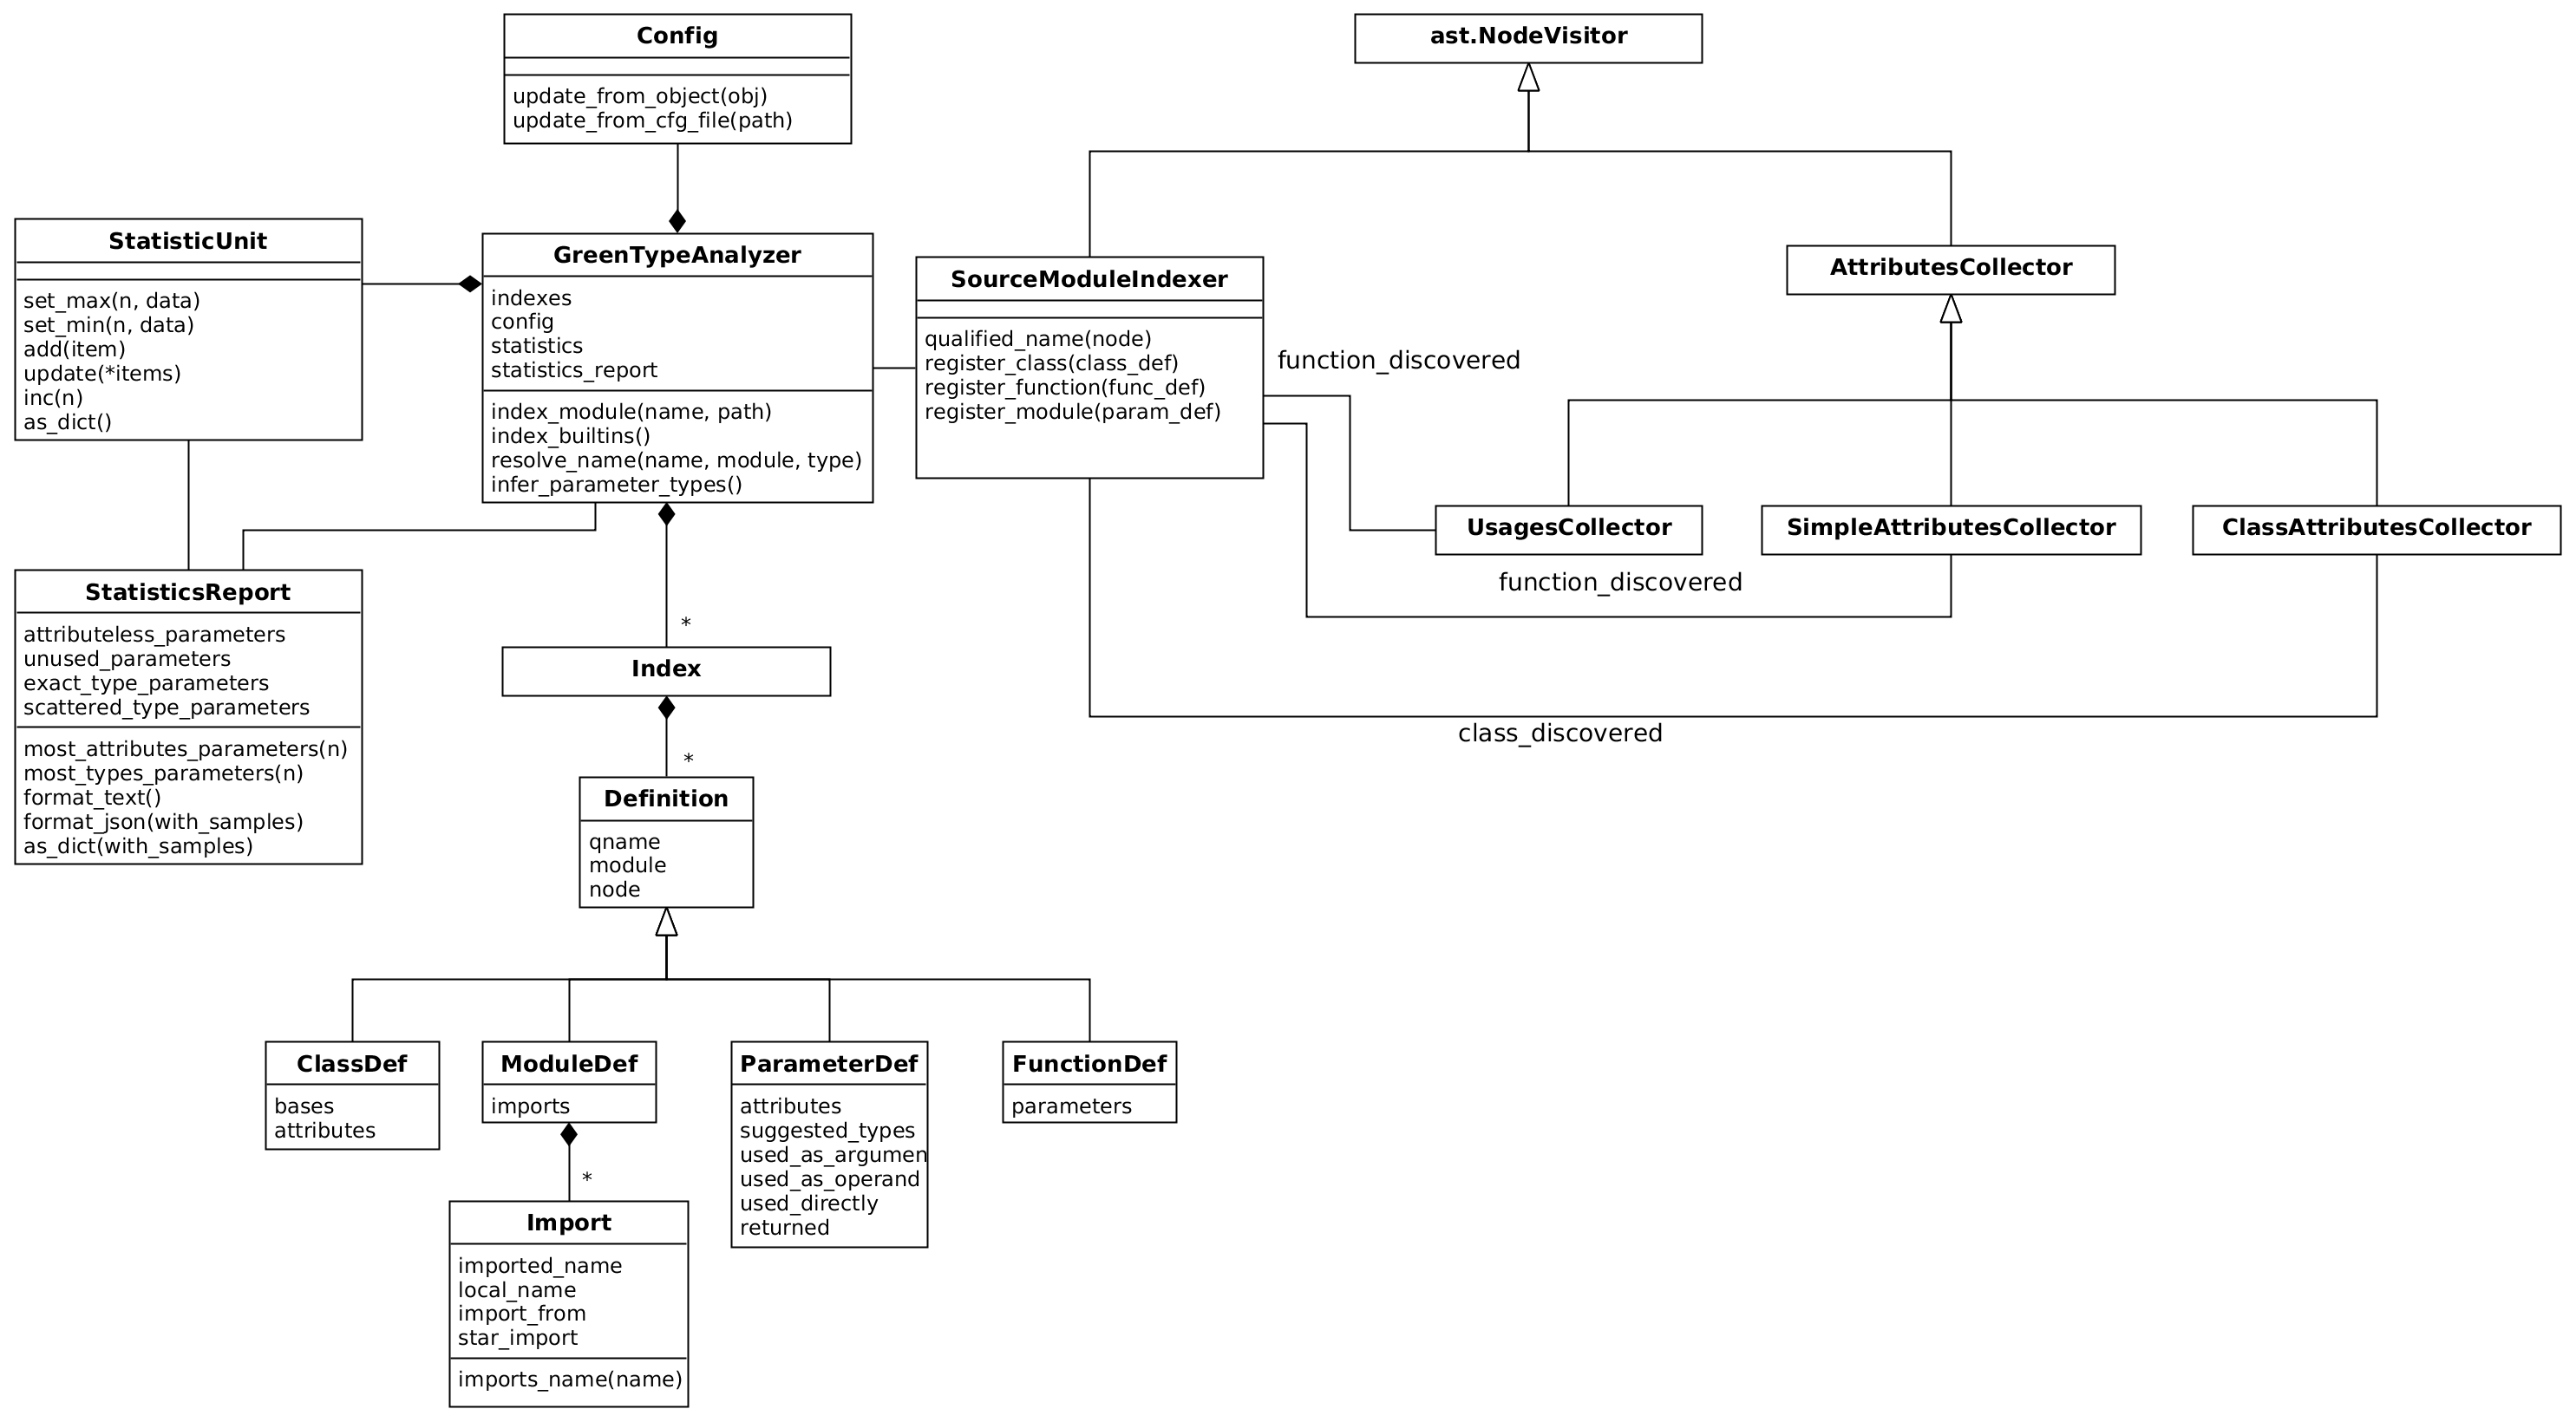
\includegraphics[width=0.85\textheight]{fig/classes-diag.png}}%
% {Диаграмма классов в проекте}{fig:classes-diag}

% Hackity-hack to left both rotated figure and title on the same page
\begin{turn}{90}
  \begin{minipage}{0.69\paperheight}
    \chapter{ДИАГРАММЫ}
    \label{app:diagrams}
    \begin{figure}[H]
      \centering
      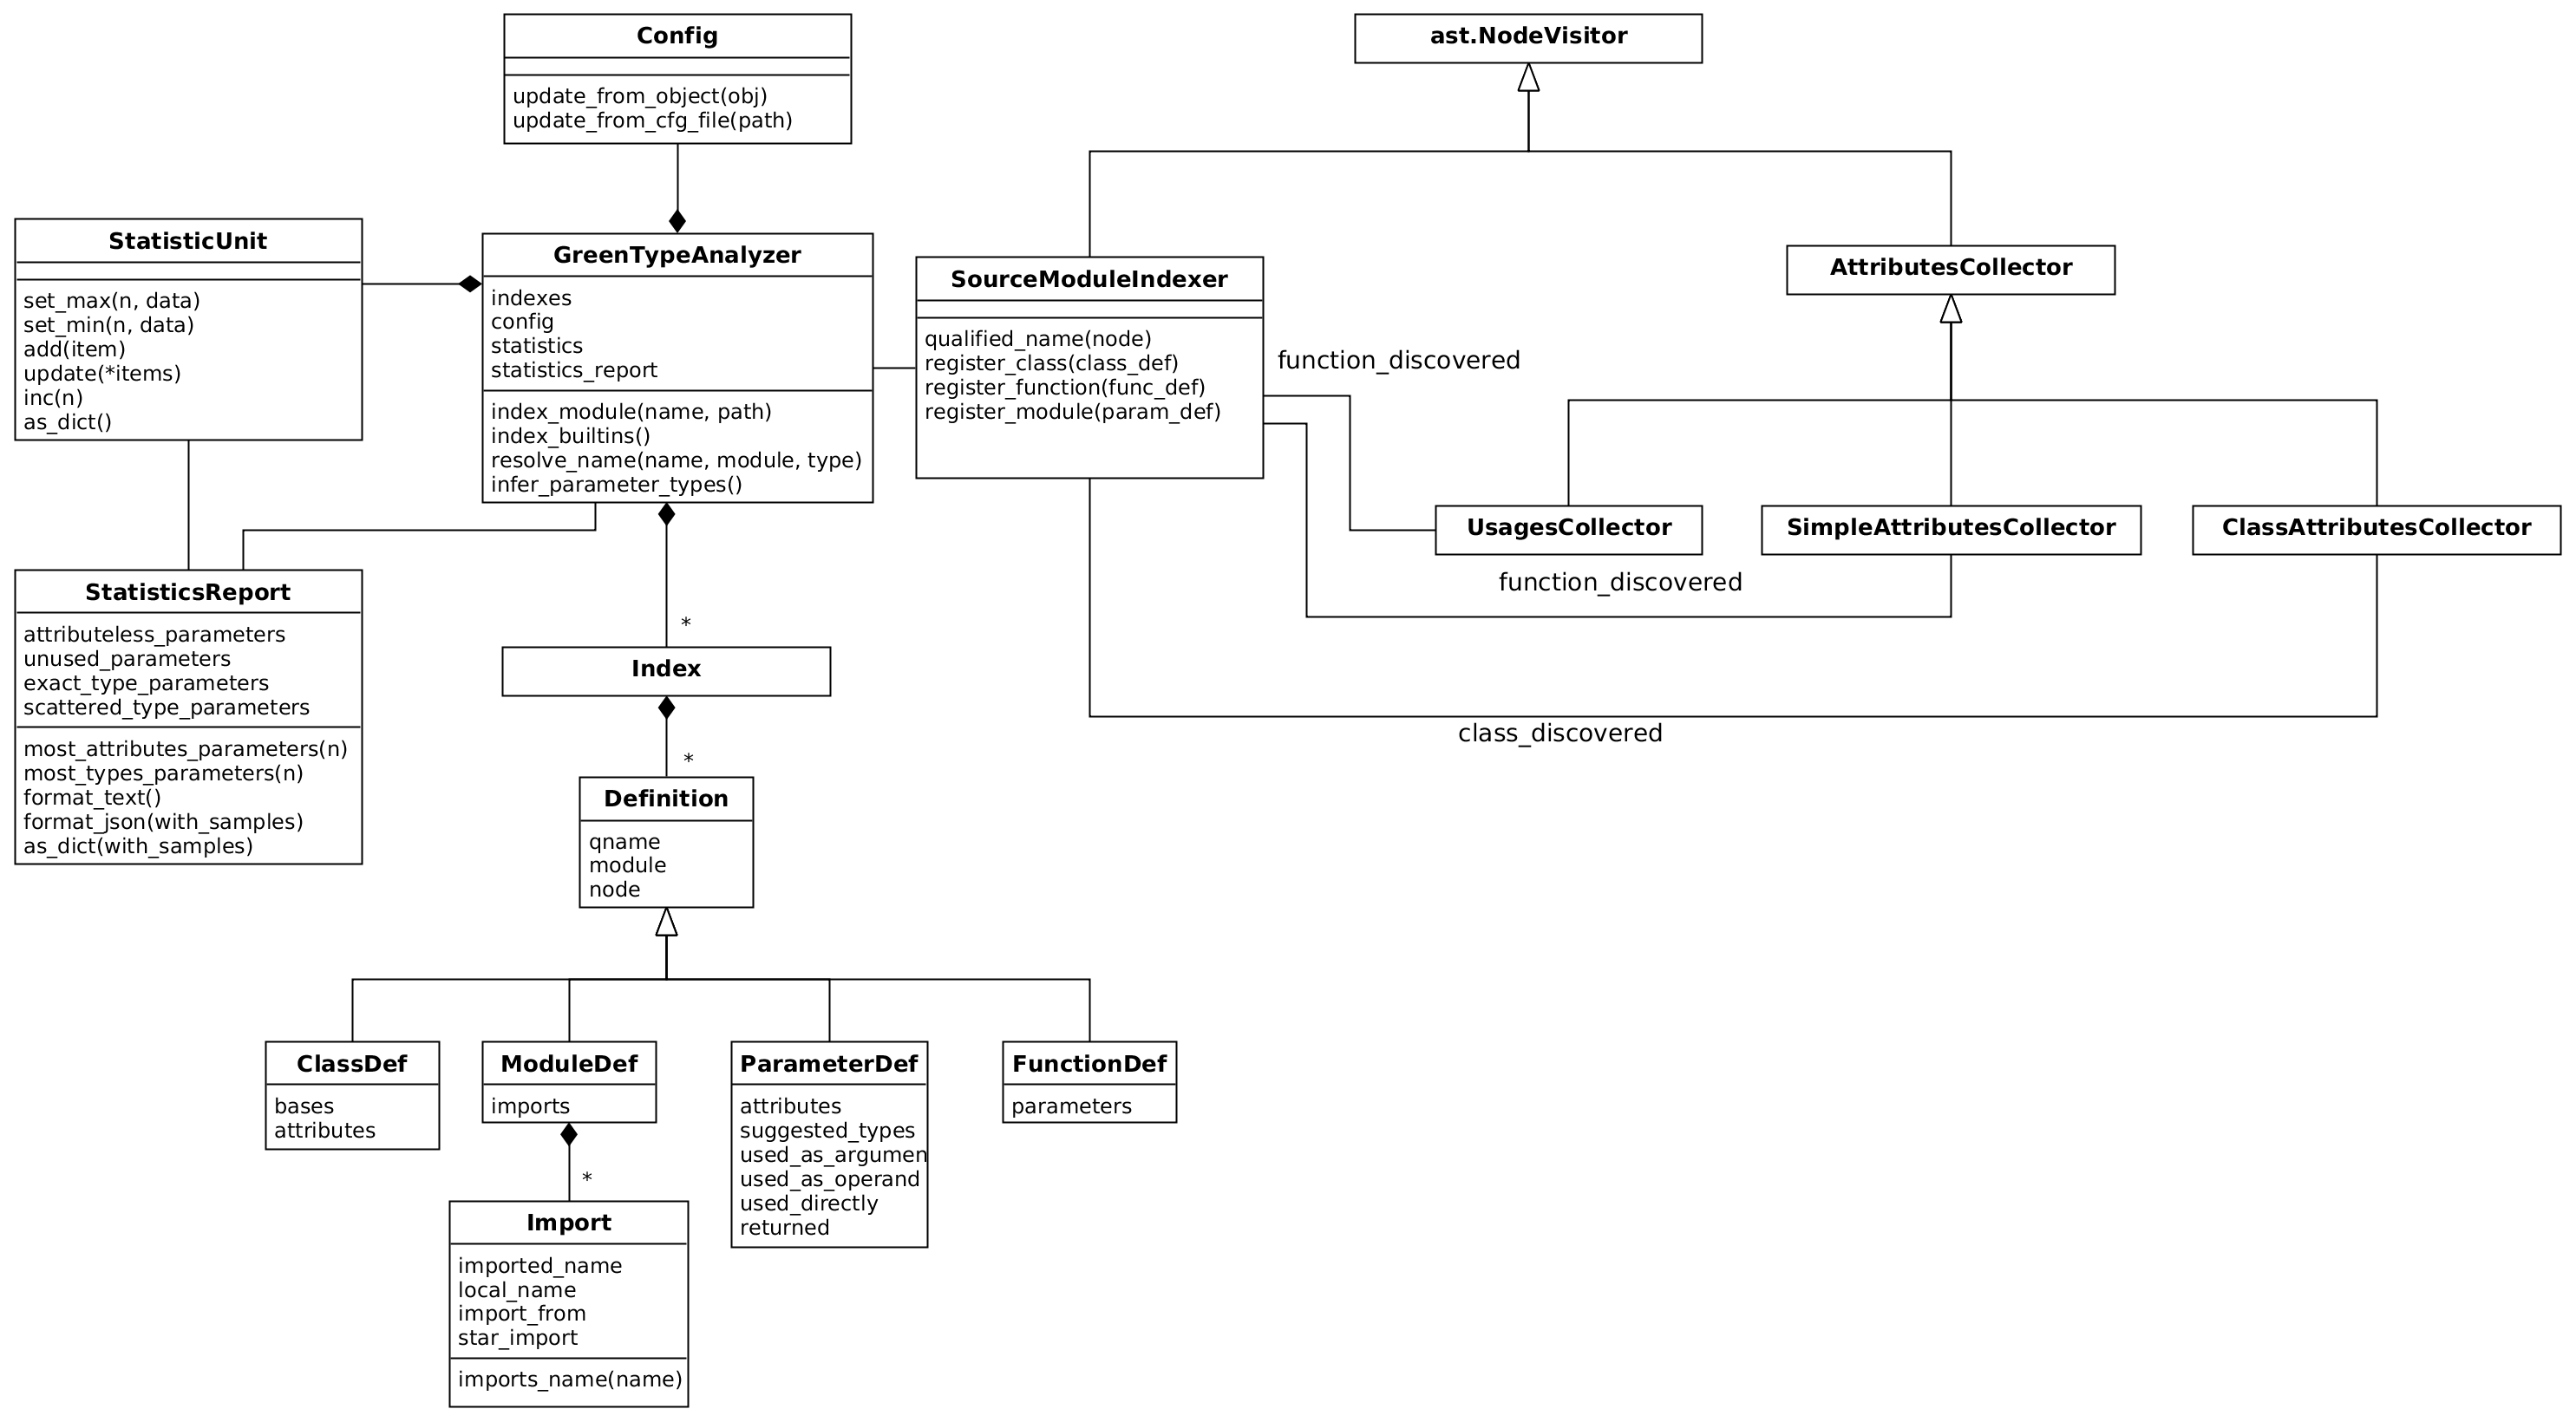
\includegraphics[width=\textwidth]{fig/classes-diag.png}
      \caption{Диаграмма классов в проекте}
      \label{fig:classes-diag}
    \end{figure}
  \end{minipage}
\end{turn}

% TODO: find out, why the heck rotfloat split title in two
% \begin{sidewaysfigure}[H]
% \begin{center}
  % 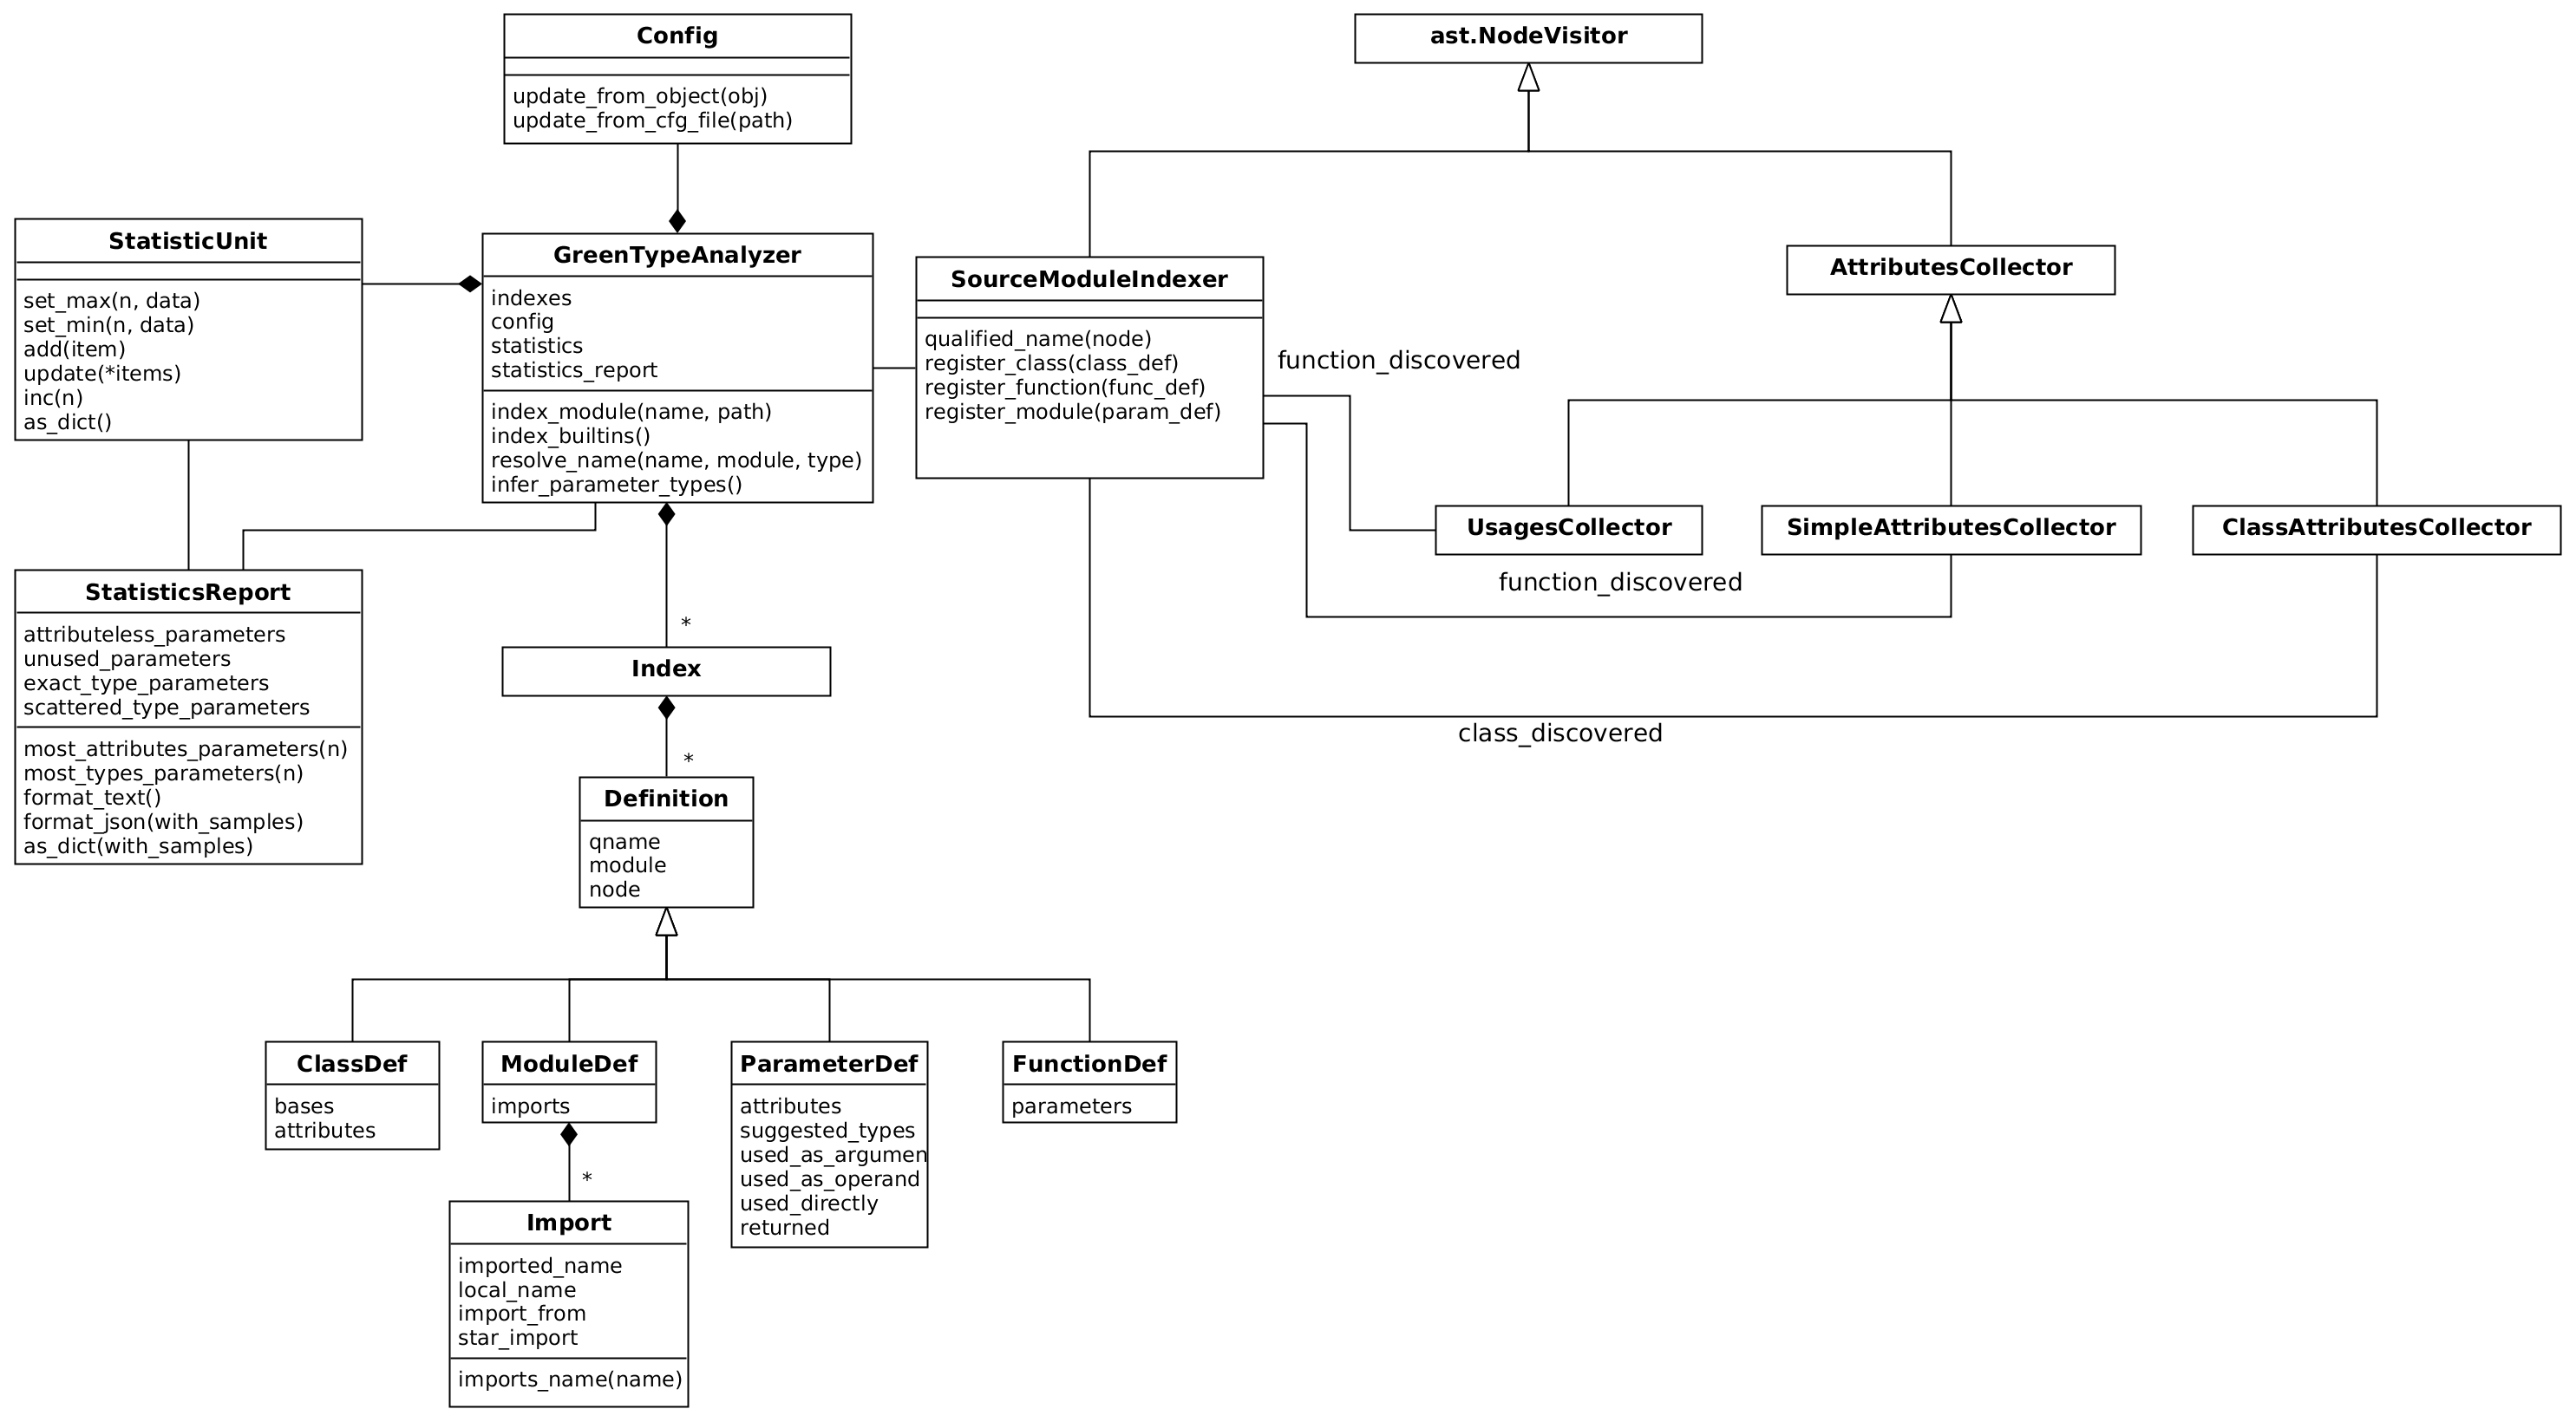
\includegraphics[width=0.8\textwidth]{fig/classes-diag.png}
% \end{center}
% \caption{Диаграмма классов в проекте}
% \label{fig:classes-diag}
% \end{sidewaysfigure}


